 %%
%% Beuth Hochschule für Technik --  Abschlussarbeit
%%
%% Hauptdokument
%%
%% 23.01.09 Tschirley V.01
%%
%%%%%%%%%%%%%%%%%%%%%%%%%%%%%%%%%%%%%%%%%%%%%%%%%%%%%%%%%%%%%%%%%%%%%
\documentclass[11pt, a4paper]{book}
%% Übersetzen als Entwurf
%\usepackage[entwurf]{bhtThesis}
%% Übersetzen für die Abgabe
\usepackage[abgabe]{bhtThesis}
\usepackage[font=small,labelfont=bf]{caption}
\usepackage{mathtools}
\usepackage{multirow,tabularx}
\usepackage{graphicx}
\graphicspath{ {./img/} }
\typeout{BHT-Abschlussarbeit V.02 15.02.12 S.Tschirley}

\usepackage{biblatex}

\usepackage{lstbayes}
\usepackage{algorithmic}
\usepackage[ruled]{algorithm2e}
\setlength\algotitleheightrule{0pt}
\SetAlgoCaptionLayout{centerline}

\makeatletter
\newenvironment{Ualgorithm}[1][htpb]{\def\@algocf@post@ruled{\kern\interspacealgoruled\hrule  height\algoheightrule\kern3pt\relax}%
\def\@algocf@capt@ruled{under}%
\setlength\algotitleheightrule{0pt}%
\SetAlgoCaptionLayout{centerline}%
\begin{algorithm}[#1]}
{\end{algorithm}}
\makeatother




\usepackage{subcaption}
\usepackage{afterpage} 
\usepackage{longtable} 
\usepackage{makecell}
\usepackage{caption}
\captionsetup[algorithm]{singlelinecheck=false}
\usepackage{pbox}
\usepackage{booktabs}
\usepackage{blindtext}   %für Blindtext in Kapitel 2
\usepackage{listings}
\usepackage{amssymb}
\usepackage{amsmath}
\usepackage{ dsfont }
\usepackage{ mathrsfs }
\usepackage{svg}

\usepackage{url}

\usepackage{color}
\definecolor{dkgreen}{rgb}{0,0.6,0}
\definecolor{gray}{rgb}{0.5,0.5,0.5}
\definecolor{mauve}{rgb}{0.58,0,0.82}


\usepackage[none]{hyphenat}
%\hyphenchar\font=-1
\sloppy

\lstset{ %
  language=R,                     % the language of the code
  basicstyle=\footnotesize,       % the size of the fonts that are used for the code
  numbers=left,                   % where to put the line-numbers
  numberstyle=\tiny\color{gray},  % the style that is used for the line-numbers
  stepnumber=1,                   % the step between two line-numbers. If it's 1, each line
                                  % will be numbered
  numbersep=5pt,                  % how far the line-numbers are from the code
  backgroundcolor=\color{white},  % choose the background color. You must add \usepackage{color}
  showspaces=false,               % show spaces adding particular underscores
  showstringspaces=false,         % underline spaces within strings
  showtabs=false,                 % show tabs within strings adding particular underscores
  frame=single,                   % adds a frame around the code
  rulecolor=\color{black},        % if not set, the frame-color may be changed on line-breaks within not-black text (e.g. commens (green here))
  tabsize=2,                      % sets default tabsize to 2 spaces
  captionpos=t,                   % sets the caption-position to bottom
  breaklines=true,                % sets automatic line breaking
  breakatwhitespace=false,        % sets if automatic breaks should only happen at whitespace
  title=\lstname,                 % show the filename of files included with \lstinputlisting;
                                  % also try caption instead of title
  keywordstyle=\color{blue},      % keyword style
  commentstyle=\color{dkgreen},   % comment style
  stringstyle=\color{mauve},      % string literal style
  morekeywords={*,...}            % if you want to add more keywords to the set
} 




%%\usepackage{hyperref}

%\usepackage[round]{natbib}

%%
%% Es folgen einige Zusätze, die in Kapitel 1 beschriben sind. 
%% Alles was nicht notwendig ist, kann auskommentiert werden
%%
\usepackage{trsym}
%\usepackage{showkeys}
\usepackage{bytefield}

\def\blankpage{%
      \clearpage%
      \thispagestyle{empty}%
      \addtocounter{page}{-1}%
      \null%
      \clearpage}

%%
%% Pfad zu den Bildern
%%
\graphicspath{
  {img/},
}

%%
%% Einbinden persönlicher macros 
%%
%
% Persönliche Macros
%
%

% Macros für Formeln
\newcommand{\jw}{j\omega}

% Begriffe

\newcommand{\OPV}{Operations\-ver\-stär\-ker}



%% Message
\typeout{-----------------------------------------------------------}
\typeout{----> main.tex ---- Zentrales Dokument---------------------}
\typeout{-----------------------------------------------------------}

\version{0.1$\alpha$}
\datum{\today}
%%
%% Titel, Autor und Betreuer
%%
\fachbereich{VI} 
\studiengang{Medieninformatik}
\autor{Sebastian Herrmann}
\edvnr{852049}
\titel{Generating Electronic Health Records: an Investigation on Gender-Medicine and Rare Diseases}
%\untertitel{Evaluating the Accuracy of Variational Bayes Variational Inference in Survival Analysis}
\betreuerFeld{
  \begin{tabular}{lr}
    \multicolumn{2}{l}{\textbf{Gutachter}}\\
    Prof. Dr.-Ing. habil. Alexander Löser & Beuth Hochschule für Technik Berlin\\
    Prof. Dr. Felix Bießmann & Beuth Hochschule für Technik Berlin
  \end{tabular}
}

%%%%%%%%%%%%%%%%%%%%%%%%%%%%%%%%%%%%%%%%%%%%%%%%%%%%%%%%%%%%%%%
%% Literaturverzeichnis

\clearpage\newpage
\addcontentsline{toc}{chapter}{References}
%\bibliographystyle{myapalike}
%\bibliographystyle{apa}
\bibliography{library}


%%\renewcommand{\baselinestretch}{1.05} 
\begin{document}
\pagestyle{fancy}
\thispagestyle{empty}
\renewcommand{\bibname}{References}

%makecell package formatting
\renewcommand\theadfont{\normalsize}
%\renewcommand\theadfont{\itshape}

\thispagestyle{empty}
\maketitle

\blankpage

\thispagestyle{empty}
\section*{Abstract}
XXX


\blankpage

\clearpage

\thispagestyle{empty}
\tableofcontents

\blankpage


\pagenumbering{arabic}
%%%%%%%%%%%%%%%%%%%%%%%%%%%%%%%%%%%%%%%%%%%%%%%%%%%%%%%%%%%%%%%





\chapter{Introduction}
% Am Anfang jedes Kapitels kurze Übersicht, was das Kapitel beinhaltet

\section{Problem}
\section{Goal}
The goal of our research is to address the issue of medGAN not taking gender into account and to further improve its generated samples' quality.
\section{Method}
\subsection{Preliminary: GAN}
TODO: SHORT DESCRIPTION OF GAN
\subsection{medGAN}
A central aspect of this work will be the application of the medical Generative Adversarial Network (medGAN), that is proposed in \cite{Choi2017}.
It is a GAN, able to generate realistic synthetic patient records. \cite{Choi2017} proofs in his work, that medGAN outperforms classical machine learning algorithms like Linear Regression, Random Forests and Support Vector Machine. 
In Chapter 2, the motivation of creating medGAN will be explained. In Chapter 4, we will provide detailed information on the architecture of medGAN and give info on recent improvements on medGAN.
\subsection{binary/count variables}
For our experiments, we generated both, records with binary and count variables. Records with binary data will show whether an ICD code occured or not, while records with count data will show how many times each ICD code occurred for each patient.
\\
\\

\begin{table}
\begin{center}
\begin{tabular}{l*{3}{c}r }
Patient ID & ICD CODE 1 & ICD CODE 2 & ICD CODE 3 \\
\hline
A & 0 & 0 & 1 \\
B & 1 & 1 & 0 \\
C & 0 & 0 & 0 \\
\hline
\end{tabular}
\caption{Example binary data entries}
\end{center}
\end{table}


\begin{table}
\begin{center}
\begin{tabular}{l*{3}{c}r }
Patient ID & ICD CODE 1 & ICD CODE 2 & ICD CODE 3 \\
\hline
A & 0 & 5 & 0 \\
B & 1 & 0 & 9 \\
C & 0 & 2 & 0 \\
\hline
\end{tabular}
\caption{Example count data entries}
\end{center}
\end{table}

\subsection{privacy risk}
The risk of hurting a patient's privacy is one of the main reasons, why Electronic Health Data is not publicly available. A commonly used method for providing access to patient data for researchers is de-identification, used for example on the MIMIC-III dataset. In this process, data gets cleansed and shifted, meaning that names, telephone numbers etc. get removed and dates are altered. \cite{johnson2016mimic}
However, \cite{Choi2017} explains that de-identification does not eliminate the risk of harming a patient's privacy, because "in certain circumstances, re-identification of patients can be accomplished through residual distinguishable patterns in various features (e.g., demographics (Sweeney, 1997; El Emam et al., 2011a), diagnoses (Loukides et al., 2010), lab tests (Atreya et al., 2013), visits across healthcare providers (Malin and Sweeney, 2004), and genomic variants (Erlich and Narayanan, 2014)) \cite{Choi2017}

On the contrary, as the synthetic data from medGAN is artificially created, there is no direct connection between the real and the synthetic samples. Therefore identifying patients from the original dataset should, intuitively, not be possible if the artificially created samples get compromised. In \cite{Choi2017} assesses the privacy risk for the case that the synthetic samples get compromised and comes to the conclusion that a potential attacker poses no risk of breaching privacy, except for when he already has significant knowledge about various features of the target patient.
\section{Outline}
This concludes Chapter 1. It explained the problem we are examining and the goal, we are trying to reach.
For giving an insight into our method, we first gave a quick insight into Generative Adversarial Networks and medGAN. Both will be explained more thoroughly in the following Chapter 2. This chapter also depicts on two examples, how the generated data will be represented. We also gave an outlook on \cite{Choi2017}'s work on investigating the privacy risk that synthetic samples pose.
This work is divided into 6 chapters, starting with 'Introduction.'
'Related Work'
'Data Analysis'
'Electronic Medical Record Generation'
'Experimental Evaluation'
'Conclusion and Outlook'
\chapter{Related Work (approx. 5-8 pages)}
\section{Abstract}
The following section will elaborate on the basic concepts that are needed to  generate synthetic electronic health record data.
First, we explain the concept of a Generative Adversarial Network. Further, we will define what exactly an Electronic Health record is. Subsequently, we will introduce the definition of Gender Medicine and Rare Diseases and their role in this work. Last, we will explain medGAN in detail.

\section{Basic Concepts}
\subsection{Generative Adversarial Networks}
In \cite{goodfellow2014generative} proposed a new framework for generative models, that learns the patterns in a given dataset and generates new data that plausibly could originate from the original dataset.
 The model Goodfellow proposes corresponds to a two-player minimax game in which two independent neural networks train simultaneously: a generator \textbf{G} which is learning the distribution of the given data and a discriminator \textbf{D} which aims to distinguish between the data from the training set and from \textbf{G}. G generates the data from the learned distribution and takes random noise as input.

In this game, G has the goal to maximize the probability of D making a mistake.  \cite{goodfellow2014generative}
\\
\\
The two-player minimax game, as shown in \cite{Goodfellow2014}, can be described by the following value function:
\\
\begin{equation}
	\min_G\max_DV(D,G) = \mathbb{E}_{x\sim{P_{data(x)}}}[log D(x)] + \mathbb{E}_{z\sim_{P_z(z)}}[log(1 - D(G(z)))]
\end{equation}
\\

For a better understanding of the process of the model, the analogy can be helpful:
"The generative model can be thought of as analogous to a team of counterfeiters, trying  to  produce  fake  currency  and  use  it  without  detection,  while  the  discriminative  model  is analogous to the police, trying to detect the counterfeit currency.  Competition in this game drives both teams to improve their methods until the counterfeits are indistinguishable from the genuine articles." \cite{goodfellow2014generative}

Mainly due to their performance in generating synthetic image data that can not be distinguished from real images, Generative Adversarial Networks gained a considerable amount of attention since their introduction in 2014.


% minGmaxDV(D,G) =Ex∼pdata(x)[logD(x)] +Ez∼pz(z)[log(1−D(G(z)))].
\subsection{Electronic Health Records}
The EHR is defined as "a longitudinal electronic record of patient health information generated by one or more encounters in any care delivery setting. Included in this information are patient demographics, progress notes, problems, medications, vital signs, past medical history, immunizations, laboratory data and radiology reports." \cite{HIMMS}
The term 'Electronic Medical Record' often is used synonymously, but a distinction between both terms has to be made.
The Office of the National Coordinator for Health Information Technology defines an EMR as the digital version of a patient's paper record. It contains time tracking data, health parameters (for example blood values), and information about checkups. They are maintained for each practice. It's intended usage is for the hospital or doctor itself and it is not meant to be shared. \cite{ONC}
EHR, on the other hand are meant to give a perspective on the overall health of each patient and to be shared for research, other healthcare providers and even the patients themselves. \cite{ONC}

- A distinction has to be made between Eletronic Health Recors and Electronic Medical records
- interoperability is not always given due to missing standards
- risk to be stolen more easily
- not centralized 
- in this work we generate a part of it: diagnosis codes
- can also be applied to medications etc. 

%eo
\subsection{Gender Medicine}
Medical research is dominated by the male gender, meaning that women are heavily underrepresented or sometimes even excluded from research studies not only in animal studies but also in human trials. \cite{baggio2013gender} 
But "diseases  differ  between  men  and  women  in  terms  of  prevention,  clinical  signs,  therapeutic  approach,  prognosis,  psychological  and  social  impact." \cite{baggio2013gender}
Sex-differences can also be found in the correlation of diseases. \cite{kautzky2010sex} shows in his research that "Sex-specific differences appear particularly relevant in the management of type 2 diabetes mellitus (T2DM), with women experiencing greater increases in cardiovascular morbidity and mortality than do men." \cite{kautzky2010sex}
Gender, however, does not only include sex, but also lifestyle-related diseases, stress, and behaviour, like, for example, regarding help-seeking actions.
While we can not take the socio-cultural aspect of gender into account, the differences in sex are applicable.
As "cardiovascular disease is the leading cause of death of both men and women" \cite{arain2009sex}, we can find numerous occurrences in the MIMIC-III dataset. This allows us to investigate the co-occurrences of diabetes and CVD.
Originally MedGAN was trained with male and female patients simultaneously, making no difference between them. In this work we are separating the dataset in order to introduce a distinction between genders.

The previously mentioned gender-differences lead us to one of our hypotheses, which will be formulated in Chapter 4.

\subsection{Rare diseases}
In Europe, a rare disease, also know as orphan disease, is defined as such when there are no more than 5 occurrences in 10.000 people. As defined by Orphanet, there are roughly 6,000 to 7,000 rare disorders, which include diseases, syndromes and anomalies. The characteristic of a disease is an altered state of health, presented "as a unique pattern of symptoms with a single treatment". \cite{Orphanet}. The majority of rare diseases have a genetic origin, but can also originate from an infection or due to unknown reasons. \cite{Orphanet} Specific codes for orphan diseases are only scarce in international classification systems like ICD-10 or ICD-9, which is used in this work \cite{rath2012representation}, resulting in a deficit of information  for researchers regarding orphan diseases. This problem finds its cause in the lack of research and a lack of awareness for rare diseases until recently, also resulting in patients without a diagnosis and unidentified illnesses. \cite{Orphanet}
Therefore Orphanet developed a nomenclature, in which each rare disease receives a unique ORPHAnumber. This system increases visibility of rare diseases and interoperability among health and research information systems. \cite{Orphanet}




\subsection{medGAN}
The wide adoption of the electronic health record system by healthcare organizations (HCOs) promises advances in analyzing patient data and computational health. The records, however, are not easily accessible for researchers. Due to the fact that EHR data consists of personal and sensitive information, access is restricted in order to not induce a privacy risk. Further, to minimize the risk of data misuse, access to such data is regulated by the HCOs. \cite{Choi2017}
(Even researches that are in direct cooperation with a hospital, do not get access to patient data.)
 As \cite{Choi2017} states, "[t]he review process by legal departments and institutional review boards can take months, with no guarantee of access (Hodge Jr et al., 1999). This process limits timely opportunities to use data and may slow advances in biomedical knowledge and patient care (Gostin et al., 2009)."
 \cite{Choi2017} describes, that "HCOs often aim to mitigate privacy risks through the practice of de-identification (for Civil Rights, 2013), typically through the perturbation of potentially identifiable attributes (e.g., dates of birth) via generalization, suppression or randomization. (El Emam et al., 2015) However, this approach is not impregnable to attacks, such as linkage via residual information to re-identify the individuals to whom the data corresponds (El Emam et al., 2011b). An alternative approach to de-identification is to generate synthetic data (McLachlan et al., 2016; Buczak et al., 2010; Lombardo and Moniz, 2008). However, realizing this goal in practice has been challenging because the resulting synthetic data are often not sufficiently realistic for machine learning tasks."  \cite{Choi2017}
 To overcome the limitations and risks of the above-stated methods, \cite{Choi2017} introduced medGAN, which implements a Generative Adversarial Network that leverages an autoencoder to overcome its limitations: the GAN generates distributed representations of patient records, while the autoencoder decodes them into actual discrete records.
 This principle and the detailed architecture of medGAN will be further explained in the section 'Electronic Medical Record Generation'.

\section{Summary}
This chapter provided an overview of fundamental concepts that need to be understood to generate electronic medical records and to evaluate our measurements.
It gave an insight into Generative Adversarial Networks, and how they will be used in this work and into the definition of Electronic Health Records and how they are distinguishable from Electronic Medical Records.
The chapter proceeded with an explanation of gender-medicine and rare diseases and their role for the evaluation process in Chapter 5. It concluded in a detailed explanation of medGAN, that will be used in Chapter 4. In the following Chapter 3, we will investigate the MIMIC-III dataset.

\chapter{Data Analysis}
Before conducting our research we performed an exploratory data analysis on the MIMICIII dataset. The goal of this analysis was to discover patterns and correlations in the data to formulate hypotheses for further analysis. "MIMIC-III [2] is a freely accessible dataset developed by the MIT lab for computational physiology utilized by numerous researchers and scholars world wide. The database consists of demographics, vital signs, laboratory tests, medications, caregiver notes, and mortality of approximately 40,000 intensive care unit patients at Beth Israel Deaconess Medical center between 2001 and 2012." \cite{arya2019exploratory}
We used pandas and numpy for the analysis and matplotlib, to display the results.
The total number of unique patients found in the dataset is 46520, consisting of 26121 male of 20399 female patients.


\begin{table}
\begin{tabular}{l|l|l|l|l}
ICD Code & Meaning & Frequency & No. of patients affected & Percent of associated patients \\
\hline
401.9 & Essential hypertension & 20703 & 17613 & 37.86\\
414.01 &  Coronary atherosclerosis & 15229 & 13480 & 28.98 \\
428.0 & Congestive heart failure &   13111 & 9843 &21.16\\
427.31 & Atrial fibrillation&    12891 & 10271 &  22.08\\
584.9 &  Acute kidney failure &  9119 & 7687& 16.52\\
250.00 & Diabetes mellitus &  9058 & 7370 & 15.82\\
272.4 & Unspecified hyperlipidemia & 8690 & 7465 & 16.05 \\
518.81 &  Acute respiratory failure & 7497 & 6719 & 14.04 \\
599.0 &   Urinary tract infection &  6555 & 5779 & 12.42 \\
530.81 & Esophageal reflux &  6326 & 5272 & 11.33\\
\end{tabular}
\caption{\label{tab:top10-codes-dataset}Top 10 of most occurring ICD9 codes in the dataset}
\end{table}


First, as a basic overview, we check for the Top10 most occurring ICD9 codes in the dataset. As depicted in \textbf{Table 3.1}, \textit{essential hypertension} has the highest frequency in MIMIC-III, followed by 3 more codes of circulatory diseases. \textit{Diabetes mellitus (DM)} can also be found in the list of the most occurring codes.

\begin{figure}
  \begin{center}
  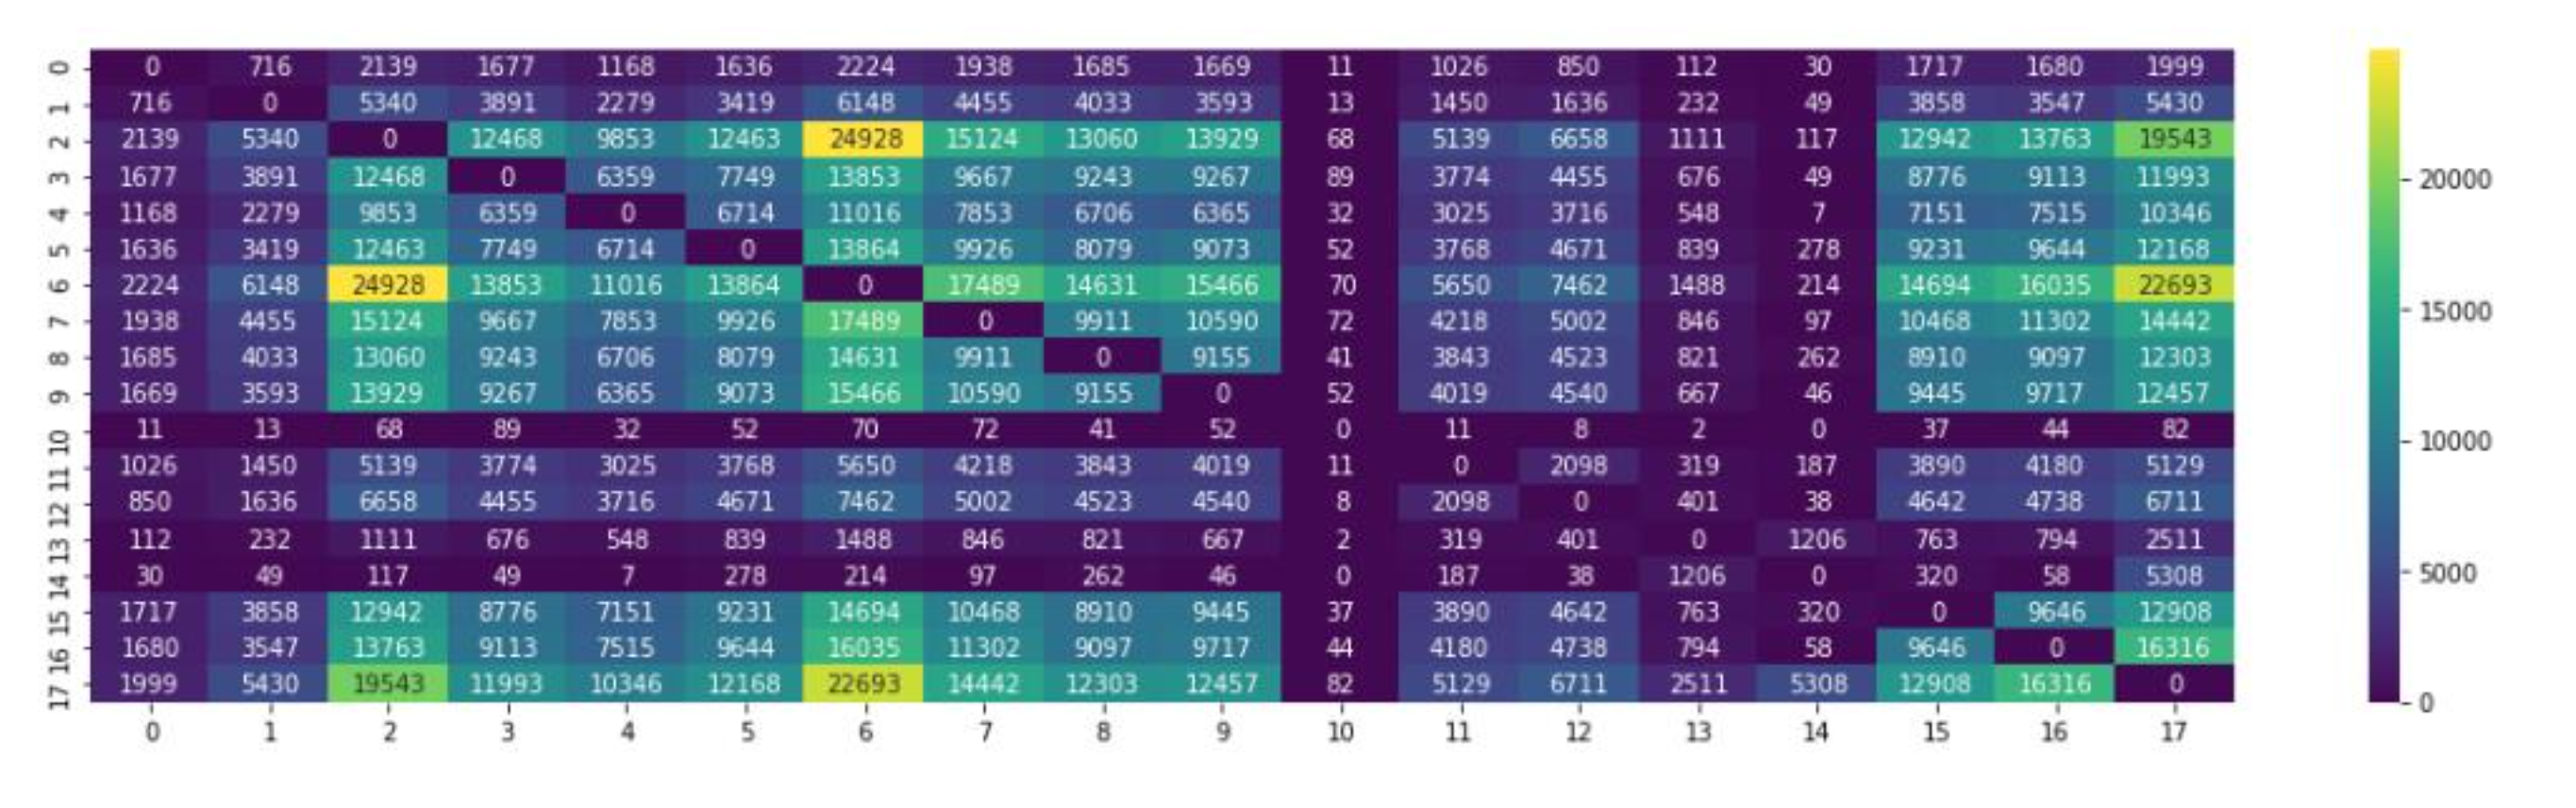
\includegraphics[width=1\textwidth]{img/correlation-heatmap.png}
  \caption{Correlation heatmap of ICD code groups \cite{arya2019exploratory}}
  \label{fig:correlation-heatmap}
  \end{center}
\end{figure}


\\
\\
Next, we have a look at the correlation heatmap (\textbf{Figure 3.1}) that is introduced in \cite{arya2019exploratory}. It shows the strongest correlation of ICD9 codes from the groups two and six, which correspond to \textit{endocrine, nutritional and metabolic diseases and immunity disorders} and \textit{diseases of the circulatory system}. Codes from group two refer to the range of codes from 240-279 , codes from group six refer to codes in the range from 390 to 459. As shown in \textbf{Table 3.1}, codes from group six are the most frequent. From group two, we can find two codes, 250.00 \textit{Diabetes mellitus} and 272.4, \textit{unspecified hyperlipidemia}.
\\
\\
Next, we proceed with comparing the top 10 occurrences of male and female diagnoses in the groups above-mentioned. We begin with the comparison of the most frequent codes of diseases of the circulatory system for male and female patients.
\\
\\
We can see that....

Subsequently, we filter all patients with coronary artery disease (Code 414.01) by diabetic diseases (Code 250.*) and compare the frequencies for male and female patients. 7280 female and 9174 male patients are affected by any form of diabetic disease.
For coronary artery disease, 3660 female and 9820 male patients are affected. 


\begin{table}
\begin{center}
\begin{tabular}{l|l|l|l|l}
Gender & diabetes & no diabetes & Total & Percentage\\
\hline
Female & 1518 & 2142 & 3660 & 41.48/58.42\\
Male 	& 2705 & 7115 & 9820 & 27.55/72.45\\
\end{tabular}
\caption{\label{tab:cad-diabetic}Patients that have CAD and diabetes and patients, that have CAD and no diabetes}
\end{center}
\end{table}


In \textbf{Table 3.1} we can see, that female patients with diabetic disease are significantly more often affected by coronary artery disease than male patients. The increased prevalence of cardiovascular diseases for women that have DM is a known risk factor, as already stated in Chapter 2.

\begin{figure}
  \begin{center}
  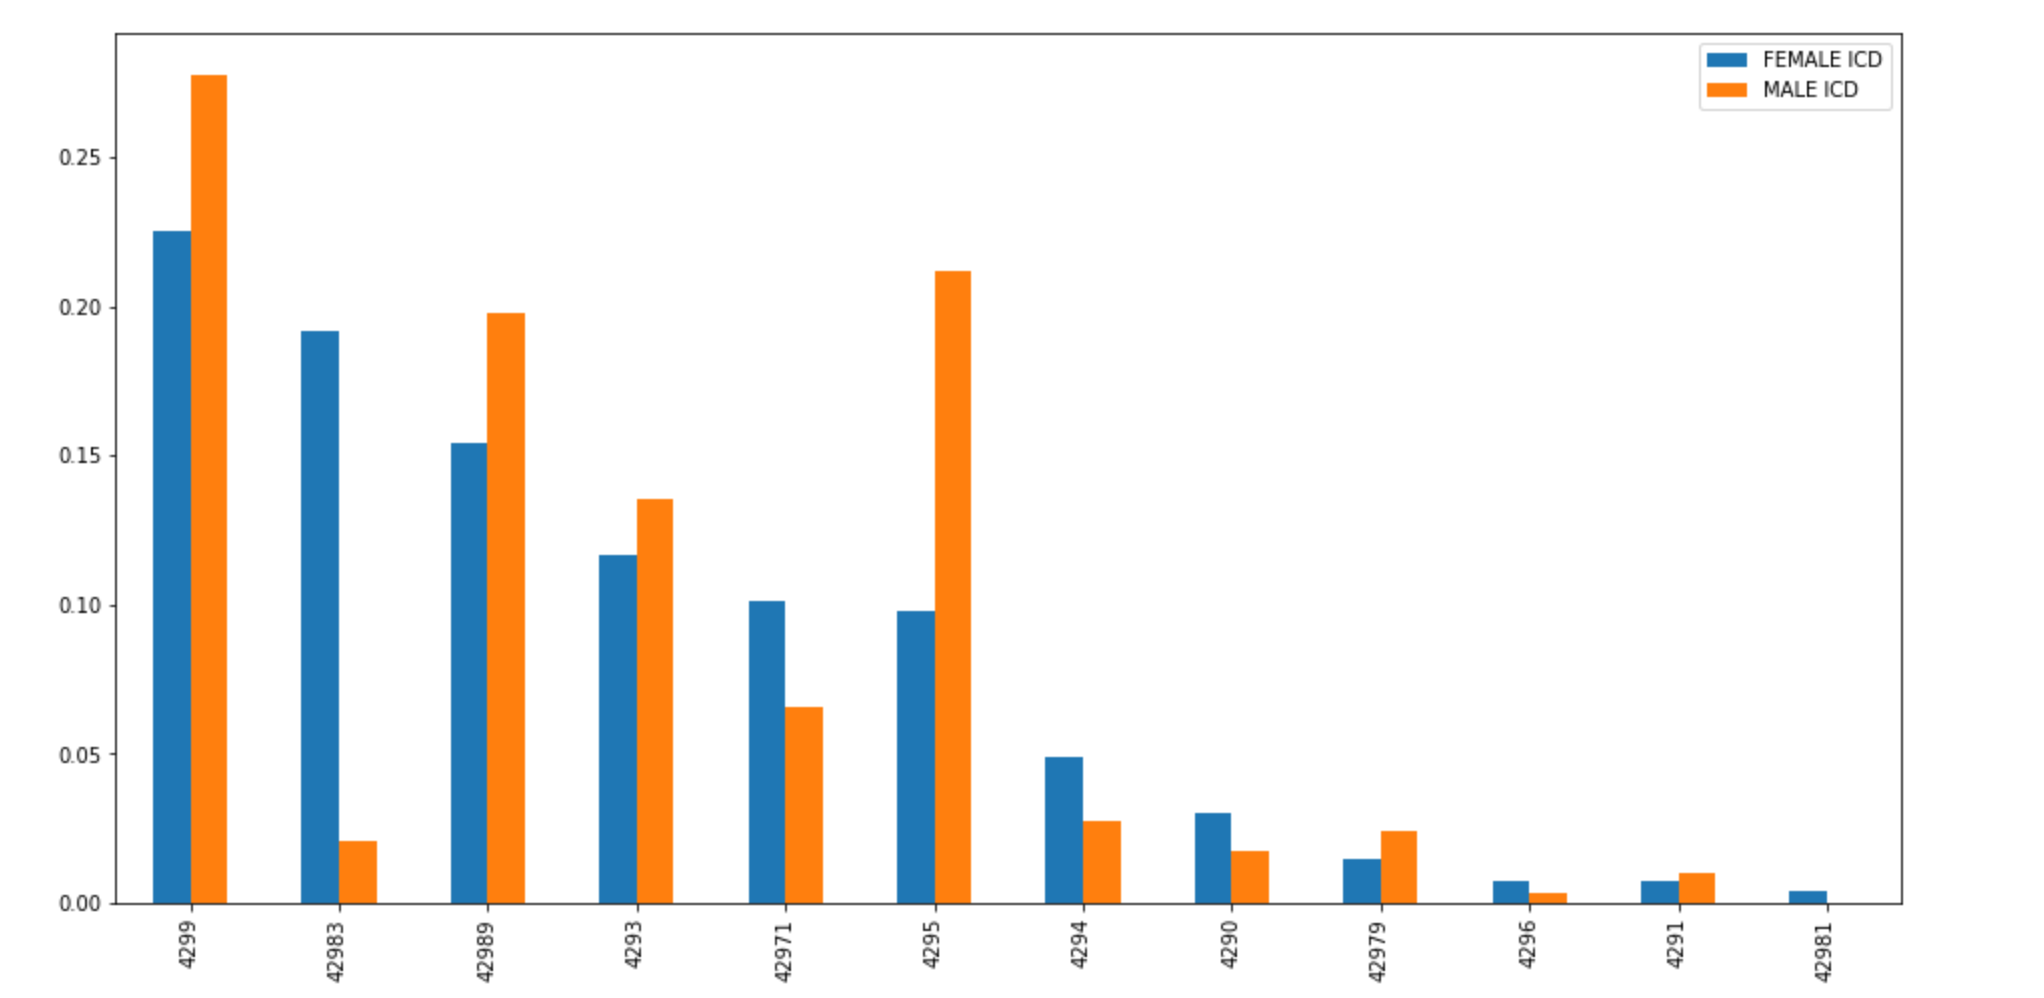
\includegraphics[width=1\textwidth]{img/male_female_heart_disease.png}
  \caption{Comparison male/female heart disease. The X axis describes the ICD9 code, the Y axis the percentage of affected patients.}
  \label{fig:heart_disease_comparison}
  \end{center}
\end{figure}

Out of 46520 patients, in our dataset 14851 female and 19185 male are diagnosed with any form of heart disease. We can see, that mostly women are affected by Takotsubo syndrome (ICD9-Code 429.9) and that around twice as many men are affected by Rupture of chordae tendineae as women (ICD9-Code 429.5). For unspecified Heart diseases (code 429.9) and other ill-defined heart diseases (code 429.89) more men are affected.  However we can find more women affected by functional disturbances following cardiac surgery and unspecified Myocarditis. 

Second, we compare males and females diagnosed with diabetic diseases: (ICD9 250.*). 7280 females and 9174 males are affected.

\begin{figure}
  \begin{center}
  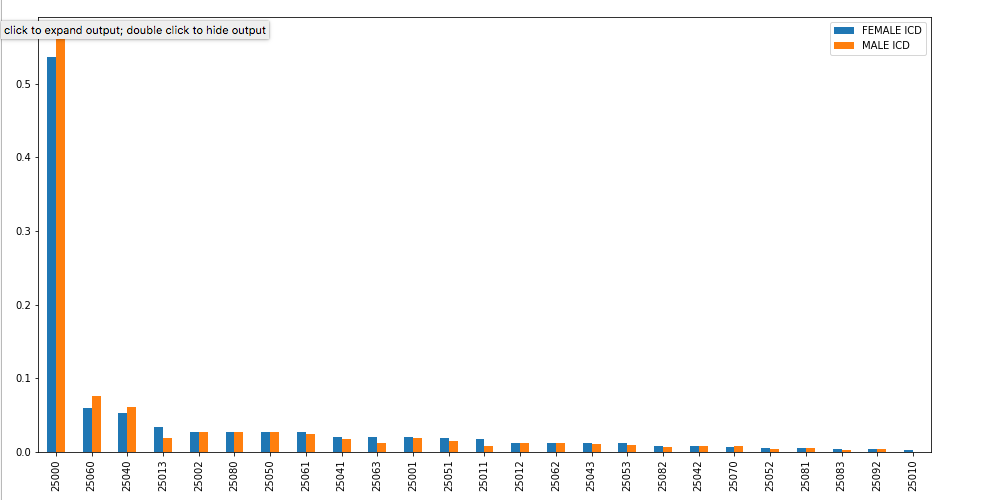
\includegraphics[width=1\textwidth]{img/comparison_diabetic.png}
  \caption{Comparison male/female diabetic disease. The X axis describes the ICD9 code, the Y axis the percentage of affected patients.}
  \label{fig:diabetic_comparison}
  \end{center}
\end{figure}

As explained in [Basic concepts - Gender medicine] correlations between diabetes and heart disease find their cause in this subject

\section{Summary}
This concludes Chapter 3. It gave an insight into the distribution of female and male patients and the most occurring ICD codes in the MIMIC-III dataset. We also learned that statistically, significantly more female patients are affected by coronary artery disease if they also have diabetic disease. This correlation is can not be found in male patients.  

\chapter{Electronic Health Record Generation}
\section{Abstract}
In this chapter, we will elaborate medGAN, discuss the process and architecture, our experimental setup and the process of training and generating synthetic Electronic Medical Record data. Further, we will introduce our hypotheses and describe the dataset.
\section{medGAN}
D and G are both implemented as feedforward neural networks.
As we learned in (SECTION GAN), the generator G "is trained by the error signal from the discriminator D via backpropagation, the original GAN can only learn to approximate discrete patient records $x \in Z|C|$ with continuous values. ” \cite{Choi2017}
To alleviate this limitation, they leveraged an autoencoder which is reconstructing an dimensionality reduced approximate of the input. As \cite{Choi2017} stated, “[s]uch a mechanism leads the autoencoder to learn salient features of the samples and has been successfully used in certain applications, such as image processing (Goodfellow et al., 2016; Vincent et al., 2008).” 

"The objective of the autoencoder is, to minimize the reconstruction error:

FORMEL AUTOENCODE
\begin{equation}
\frac{1}{m}\big[\sum_{i=0}^m \mid\mid x_i - x_i'\mid\mid_2^2]
\end{equation}
\begin{equation}
\frac{1}{m}\big[\sum_{i=0}^m x_i \log x'_i + (1-x_i) \log (1-x'_i)]
\end{equation} 
\begin{center}
where $x'_i = Dec(Enc(x_i))$
\end{center}

FORMELN STIMMEN NOCH NICHT
where m is the size of the mini-batch." \cite{Choi2017}
\\
\\
An autoenconder consists of of two elements: The Encoder (Enc) which compresses the input and the Decoder (Dec) that is used to construct the output.
For count variables they used the cross entropy loss and rectified linear units  as activation function for the Enc and Dec.
For binary variables they used the mean squared loss and the tanh activation function for Enc and the sigmoid activation for Dec.
Both, the Enc and the Dec are implemented as single layer feedforward networks. The original input x it receives, is compressed into a 128 dimensional vector. The generator G consists of two hidden-layers with each 128 dimensions and is implemented as a feedforward network. For the batch normalization in G they use the scale parameter  $\gamma$ and the shift parameter $\beta$ and set the moving average decay to 0.99. The discriminator D has the same structure, but the first hidden-layer consists of 256 dimensions. medGAN is trained for 1,000 epochs with the mini-batch of 1000 records. \cite{Choi2017}
\begin{figure}
  \begin{center}
  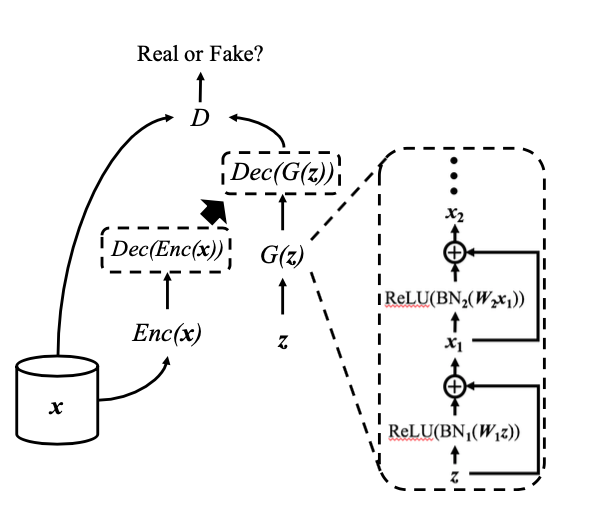
\includegraphics[width=0.5\textwidth]{img/medgan-architecture.png}
  \caption{Architecture of medGAN: The discrete x comes from the source EHR data, z is the random prior for the generator G; G is a feedforward network with shortcut connections (right-hand side figure); An autoencoder (i.e, the encoder Enc and decoder Dec) is learned from x; The same decoder Dec is used after the generator G to construct the discrete output. The discriminator D tries to differentiate real input x and discrete synthetic output Dec(G(z)).  \cite{Choi2017}}
  \label{fig:transfer_learning_no}
  \end{center}
\end{figure}

"medGAN generates synthetic EHR datasets that achieve comparable performance to real data on many experiments including distribution statistics, predictive modeling tasks and medical expert review."

UMFORMULIEREN (zitiert)

\subsection{SynthEHR (medBGAN, medWGAN)}
In \cite{Baowaly2018} proposed two altered versions of medGAN that outperform their predecessor, however just slightly.
Those two versions are:

\textbf{medWGAN}: This version substitutes the regular GAN with an improved \textit{Wasserstein GAN (WGAN)}, that utilizes "an alternative method of weight clipping called gradient penalty, which entails penalizing the norm of the gradient of the discriminator (critic) with respect to its input" \cite{Baowaly2018}

\textbf{medBGAN}: This version substitutes the regular GAN as well, but this time with a \textit{boundary-seeking GAN (BGAN)}. This approach trains the generator to match the target distribution that converges toward the true distribution as the discriminator is optimized" \cite{Baowaly2018}
\subsection{Differentiation}
Bereits erklärt?
\subsection{Why left out?}
If our hypotheses proof to be true and bring an improvement to medGAN, these improvements will also translate to altered versions of medGAN, because not the network itself is being changed but the input. In our tests we separated the dataset and did not alter it. Henceforth we performed our tests only on the 'original' medGAN. 
\section{Process and Architecture}
For generating the Electronic Medical Records (EMR), we used a Generative Adversarial Network (GAN) called medGAN, that was proposed in \cite{Choi2017}. As input data we use v1.4 of the MIMIC-III (Medical Information Mart for Intensive Care) dataset. For our experiments, we divided the dataset by gender and generated EMR data with binary and count variables for both mixed and separated patients. The code for medGAN is publicly accessible under https://github.com/mp2893/medgan. It is implemented using TensorFlow
For training models, they chose the Adam-optimizer with a mini-batch size of 100 patients. \cite{Choi2017} We trained the model using Colaboratory by Google, which is a Jupyter notebook environment, providing free Cloud computing for education and research.
The machines are equipped with K80 GPUs from NVIDIA.
With the K80 GPU, it took 29 minutes and 3 seconds to train the model with only female patients, 35 minutes and 26 seconds to train the model with only male patients and 60 minutes and 1 second to train the model with the full dataset.
\section{Experimental Setup}
 For training, we split the data into subsets with a ratio of 9:1 for training and validation subsets. Using the training subset, the autoencoder is pretrained for 100 epochs. 
 After each epoch, we report the training and validation loss. For binary variables we use the cross-entropy loss  function, for count variables the mean squared error.
 Further, we use minibatch averaging and batch normalization
We conducted our data analysis in a Jupyter Notebook. Here, we use pandas to investigate the data and matplotlib to show our results.
After finishing the training process, we select the epoch closest to 0.5, since that is when the discriminator is most confused and the generator makes the most convincing synthetic samples.


\section{Hypothesis}
In this work we are trying to proof the following three hypotheses:

First, the model can generate realistic patients if it is trained with the MIMIC III dataset / the model learns the distribution of ICD9 codes.
Second, by training the network with female and male patients separately, it is able to generate patients with gender-specific correlated diseases that seem realistic to a medical doctor.
Third, if the network is being trained with the MIMIC-III dataset, it is able to generate patients affected by orphan diseases that can not be distinguished to a non-synthetic patient by a medical doctor



\section{Data}
The dataset is publicly available for researchers worldwide. In order to gain access to it we were required to complete the CITI “Data or Specimens Only Research” course.

It contains deidentified health-related data associated of over forty thousand patients who stayed in critical care units of the Beth Israel Deaconess Medical Center in Boston between 2001 and 2012.

We extracted the ICD9 codes for female and male patients from the dataset separately and aggregated a patient’s longitudinal record into a single fixed-size vector  x elem Z{$^C$}. For ICD9-Codes shortened to 3 digits, $C$ equals 1071 for mixed patients, 987 for female patients and 966 for male patients. For, full-length 5 digits ICD9-Codes $C$ equals 6985 for mixed patients, 5650 for female patients and 5853 for male patients.

TODO: GLEICHUNGEN

Model for comparison: 

To assess the effectiveness of my method, I trained the network both, with mixed and gender-separated patients. 

\cite{Choi2017} also compared medGAN with other popular generative methods like Random Noise, Independent Sampling. In his experiments, medGAN outperformed other methods. Therefore we will compare our results with medGAN.

\section{Models for Comparison}
For our baseline we choose medGAN as proposed in \cite{Choi2017}. As stated in the paper, medGAN outperformed machine learning models like Linear Regression and Random Forests.
For our evaluation we will also use \textbf{Linear Regression} in order to indirectly measure how well the model learned interdimensional relationships.
\section{Measurements}
For comparison we generated samples of sizes, equal to the dataset.

\section{Summary}

\section{Non-Gender-specific EMR Generation}
First, like in \cite{Choi2017} we generated EMR data, without dividing the dataset. The results serve as baseline for the performance and will be compared with the separately generated patients.
\\
\\



\section{Gender-specific EMR Generation}
Second, we divided our dataset by gender and generated patient data separately, resulting in 20399 female and 26121 male unique records.
\\
%\section{Rare diseases}
Wikidata provides a mapping of 4584 ICD-9 codes to GARD and OrphaNet IDs.
To investigate the occurrence of rare diseases in MIMIC-III, we first generated a list containing all 6985 unique ICD9 codes of the dataset. Then, we match the list from the mapping which contains a total of 962 codes, resulting in ten corresponding codes in the MIMIC-III dataset. 2408 diagnoses with orphan ICD9-codes are present in the given dataset.

The following section will elaborate our findings regarding rare diseases in our generated patients.
\chapter{Experimental Evaluation}
\section{Abstract}
In the following section we will evaluate our experiments in order to measure our success. First, in a quantitative manner, using statistical methods. Second, by evaluation in a qualitative manner, comparing the generated data to the original dataset and with the help of a medical doctor.
\section{Hypotheses}
In our work we are trying to proof the following hypotheses:
First, we are making the assumption that the model can generate realistic patients if it is trained with the MIMIC III dataset and that the model learns the distribution of ICD9 codes from the dataset.
Second, by training the network with female and male patients separately, it improves on its ability to generate patients with gender-specific correlated diseases that seem realistic to a medical doctor.
Third, if the network is being trained with the MIMIC-III dataset, it is able to generate patients affected by rare diseases that can not be distinguished to a non-synthetic patient by a medical doctor.
\section{Measurements}

\section{Evaluation}
\subsection{Abstract}
In this section we will evaluate our measurements in a quantitative and qualitative manner. We evaluate the measurements for 3 digit (shortened) and 5 digit (original) ICD9-codes for both, binary and count variables.
First comes the quantitative evaluation of our generated records. For this we choose two statistical methods: dimension-wise probability for binary variables and dimension-wise average for count variables.
Second we perform the qualitative evaluation. We begin with investigating the data, like we did with the real dataset. In the next step, we are looking for correlations of diabetic-disease and heart-disease. Subsequently, we evaluate our measurements with the help of a medical doctor.
\subsection{Quantitative Evaluation}
In this section we evaluate the model's performance. For the quantitative evaluation of our measurements we choose the following statistical methods, as presented in \cite{Choi2017}.
\\
\\
\textbf{Dimension-wise probability}: This refers to the Bernoulli success probability of each dimension (disease or procedure code) in the binary dataset. The dimension-wise probability is computed using the following formula: 

\begin{equation}
Number\,of\,patients = \frac{Number\,of\,patients\, who \,had \,the \,disease}{Total \,number \,of \,patients}
\end{equation}

We calculate it for the binary data.
\\

\textbf{Dimension-wise average}: This refers to the column average of each dimension (disease or procedure code) in the count dataset. The dimension-wise average is calculated using the following formula: 
\begin{equation}
Dimension-wise\,average = \frac{Column \,sum}{Total \,number \,of \,records}
\end{equation}

We calculate it for the count data.
\\

\textbf{Dimension-wise prediction}: As stated in \cite{Choi2017}, to indirectly measure the extent of the model learning interdimensional relationships, \textbf{Logistic Regression} can be used. Therefore, we choose one dimension k of each dataset, synthetic and real, to be the label and the remaining  ones as features to train two logistic regression classifiers to predict $\gamma_R_k$ and $\gamma_S_k$
For both, dimension-wise probability and dimension-wise average, we present the outcomes in a scatterplot. Each dot represents a diagnoses code. The x-axis represents the codes from the real data, the y-axis the one's from the synthetic data.
\\
\\
For both, dimension-wise probability and dimension-wise average, we present the outcomes in a scatterplot. Each dot represents a diagnoses code. The x-axis represents the codes from the real data, the y-axis the one's from the synthetic data.
\\
\\
\textbf{Dimension-wise K–S test}: We performed the K–S test on 2 data samples (synthetic data and real data) to examine whether the 2 data samples originate from the same distribution. In the K–S test, the statistic is calculated by finding the maximum absolute value of the differences between 2 samples’ cumulative distribution functions. The null hypothesis is that both samples originate from a population with the same distribution. In our experiment, we rejected the null hypothesis with a low P-value (typically 􏰆 0.05). More details of the K–S test is discussed in the Results section. 

\begin{figure}
\centering
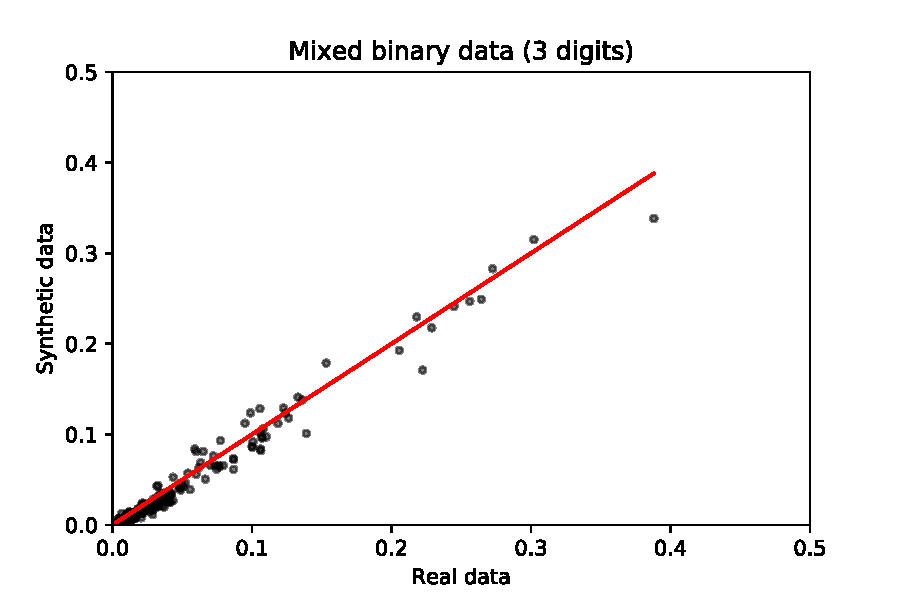
\includegraphics[width=.3\textwidth]{img/plots/binary_3digit_mixed}\hfill
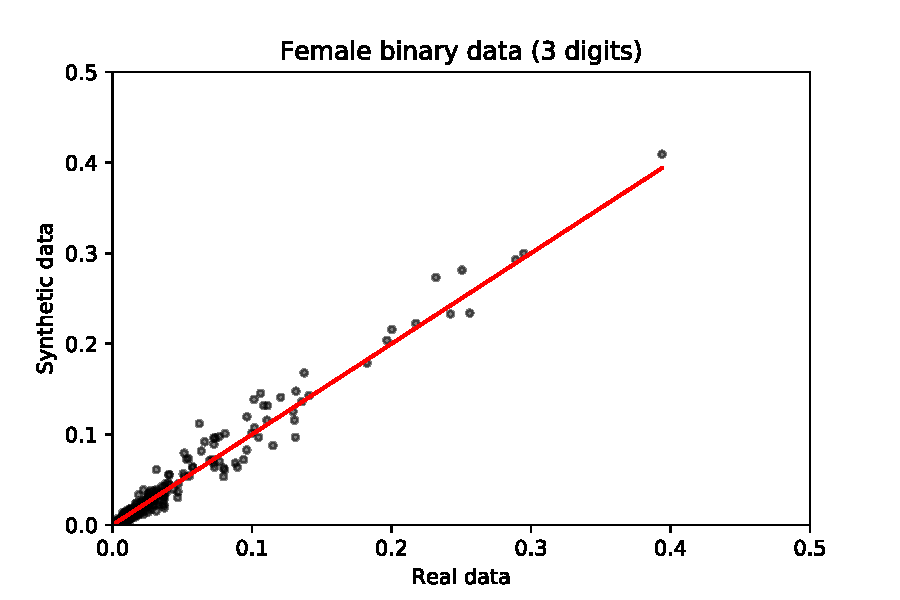
\includegraphics[width=.3\textwidth]{img/plots/binary_3digit_female}\hfill
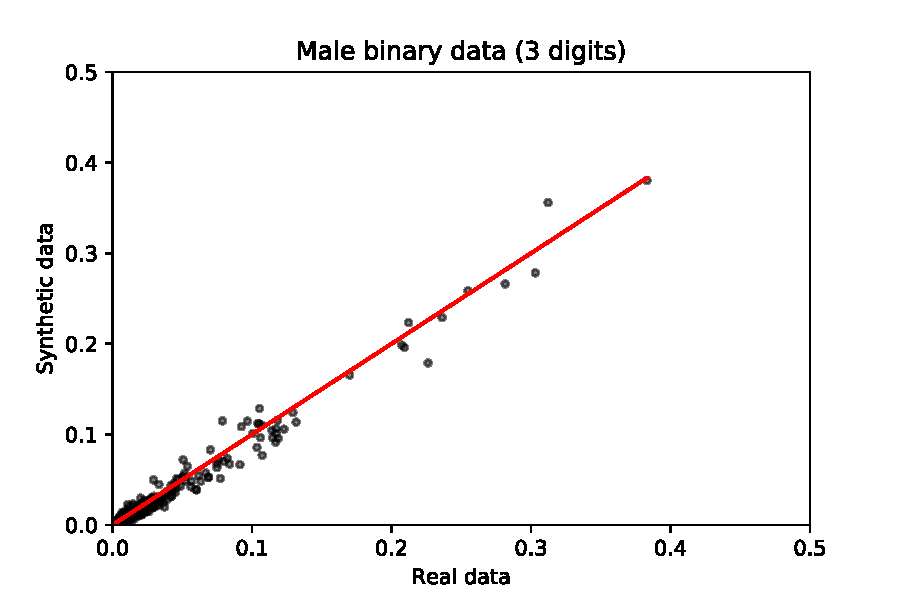
\includegraphics[width=.3\textwidth]{img/plots/binary_3digit_male}\hfill
\\
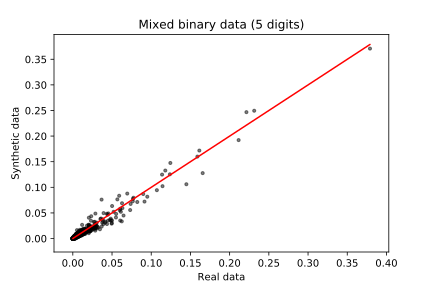
\includegraphics[width=.3\textwidth]{img/plots/binary_5digit_mixed}\hfill
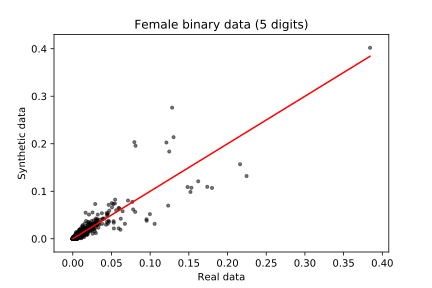
\includegraphics[width=.3\textwidth]{img/plots/binary_5digit_female}\hfill
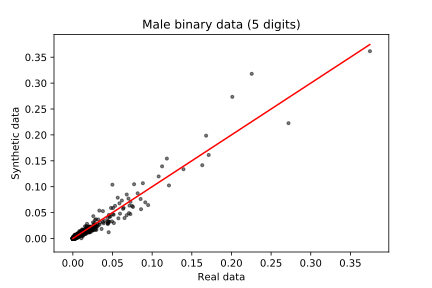
\includegraphics[width=.3\textwidth]{img/plots/binary_5digit_male}\hfill
\caption{dimension-wise probability}
\begin{flushleft}
\small
Scatterplots of dimension-wise probability. For the 3 digit codes, each dot represents one of 1071 codes for mixed samples, 987 for female samples and 966 for male samples. For the 5 digit codes, each dot represents one of 6985 codes for mixed samples, 5650 for female samples and 5853 for male samples. The x-axis represents the probability for codes from the real dataset, while the y-axis represents these from the synthetic dataset.
\end{flushleft}
\label{fig:figure3}
\end{figure}

\subsubsection{binary data}
After splitting up the dataset by gender, the performance decreased for generating both, male and female samples, while male samples are not affected as heavily. However, we can see that the performance loss is more significant, if we use the 5 digit ICD-codes. 



\\
\\
\begin{figure}
\centering
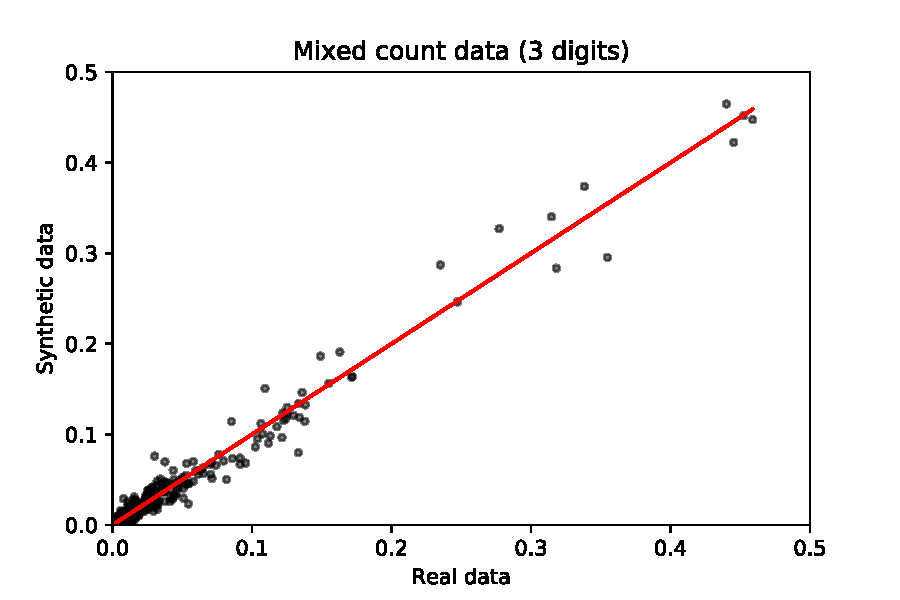
\includegraphics[width=.3\textwidth]{img/plots/count_3digit_mixed}\hfill
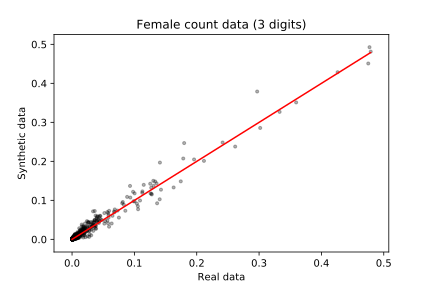
\includegraphics[width=.3\textwidth]{img/plots/count_3digit_female}\hfill
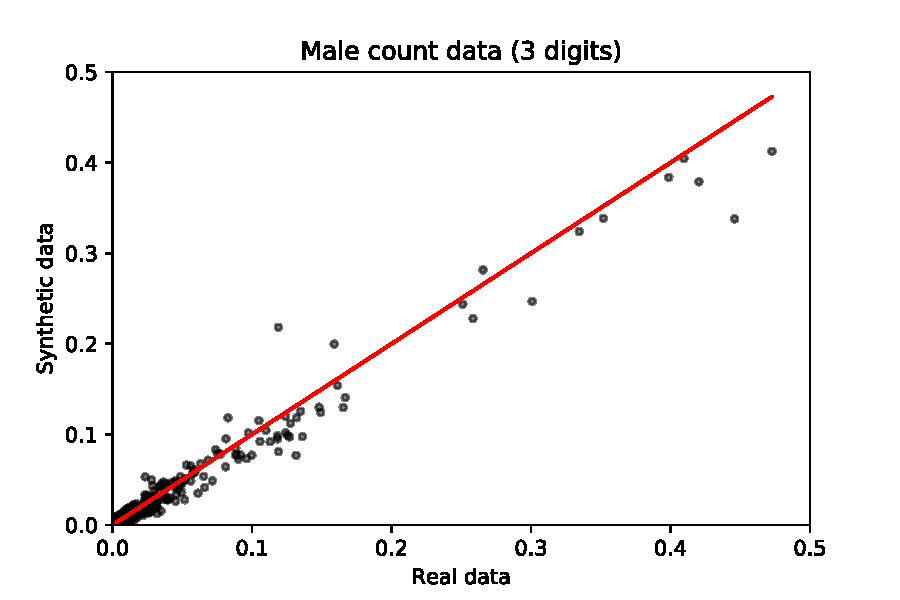
\includegraphics[width=.3\textwidth]{img/plots/count_3digit_male}\hfill
\\
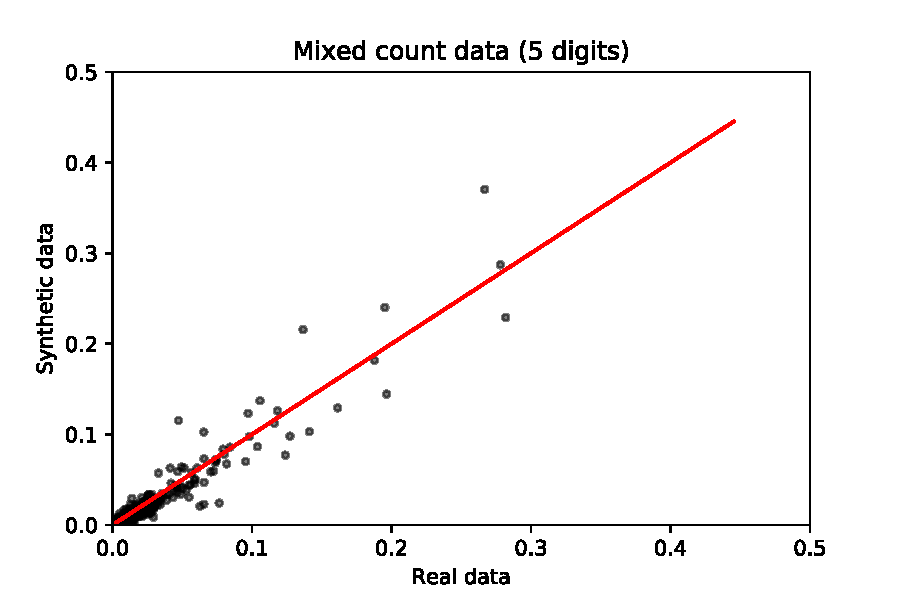
\includegraphics[width=.3\textwidth]{img/plots/count_5digit_mixed}\hfill
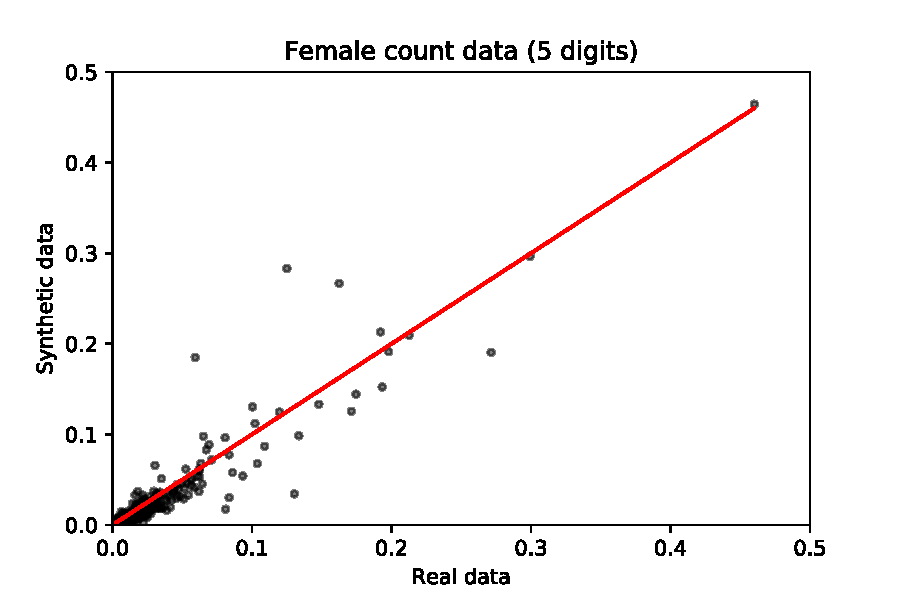
\includegraphics[width=.3\textwidth]{img/plots/count_5digit_female}\hfill
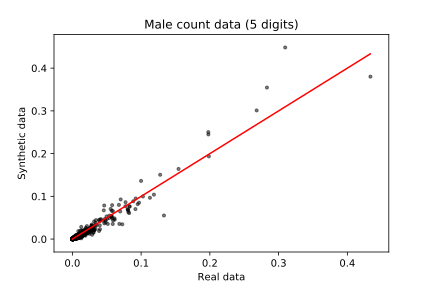
\includegraphics[width=.3\textwidth]{img/plots/count_5digit_male}\hfill
\caption{dimension-wise average}
\small
\begin{flushleft}
Scatterplots of dimension-wise average. For the 3 digit codes, each dot represents one of 1071 codes for mixed samples, 987 for female samples and 966 for male samples. For the 5 digit codes, each dot represents one of 6985 codes for mixed samples, 5650 for female samples and 5853 for male samples. The x-axis represents the probability for codes from the real dataset, while the y-axis represents these from the synthetic dataset.
\end{flushleft}
\label{fig:figure3}
\end{figure}

\subsubsection{Evaluation Orphan diseases}
For evaluating our measurements for generated patients with rare diseases, we depict our results in a table with numbers of total occurrences, since we want to find out whether the model learns to generate them at all. 
Therefore we choose the binary data for evaluation.
For this case, the qualitative evaluation is of higher importance, since we have to find out, whether the generated samples seem realistic to a medical doctor.


\textbf{Orphan diseases}:
\\
\\
\begin{table}
\begin{tabular}{l|r|r|r}
ICD9-Code & Female Binary & Male Binary & Mixed\\
\hline
042 Human immunodeficiency virus [HIV] disease	& 17 & 440 & 373\\
515 Postinflammatory pulmonary fibrosis & 124 & 44 & 117\\
570 Acute and subacute necrosis of liver & 538	& 359 & 870\\
\end{tabular}
\caption{\label{tab:rare-generataed}successfully generated samples with rare diseases}
\end{table}
\\
\\
\begin{table}
\begin{tabular}{l|r|r}
ICD9-Code & Dataset Female & Dataset Male\\
\hline
075 Infectious mononucleosis & 7 & 4\\
138 Late effects of acute poliomyelitis & 36 & 37 \\
193 Malignant neoplasm of thyroid gland & 21 & 28 \\
220 Benign neoplasm of ovary & 25	& 0\\
317 Mild intellectual disabilities & 43 & 39\\
8832 Open wound of finger(s), with tendon involvement & 2 & 15\\ 
\end{tabular}
\caption{\label{tab:rare-not-generated}rare diseases with no generated samples}
\end{table}

In Table 5.1 we see, that our model only successfully generates samples with 3 out of the 10 rare disease codes that exist in the original dataset.
Table 5.2 depicts the number of occurrences of each code in the original dataset. Here we can see, that the diseases that have been generated have over 500 occurrences and that the model  does not generate samples with codes, that have less than 100 occurrences in the input dataset.

\subsection{Qualitative Evaluation}
Our qualitative evaluation consists of three parts. First, we repeat the steps of our data analysis and compare our synthetic samples with it. Second, we investigate on synthetic dataset whether the model learned gender-specific correlations of diseases and whether it learned to generated sample patients with rare diseases. This can be seen as a further test that proofs whether the model learned the interdimensional relationships. Third, we rate our measurements with the help of a medical doctor. Therefore we take 25 samples from the original dataset and 25 samples from our generated patients. Then, we present them in random order to a medical doctor and let him rate them on realisticness on a scale from 1 to 10, where 10 is the highest score and therefore a sample, that can not be distinguished from a real record.
The samples are selected randomly, except for the rare diseases. Here we choose 5 samples each from the dataset and from our generated patients because of their scarcity.

\subsubsection{Data analysis}

\begin{table}
\begin{tabular}{l|l}
\textbf{ICD9-Code} & \textbf{Percent of affected patients}\\
\hline
401.9 Unspecified essential hypertension & 26.20\%\\
427.31 & \%\\
244.9 & \%\\
305.1 & \%\\
424.1 & \%\\
414.01 & \%\\
V58.61 & \%\\
V05.3 & \%\\
250.00 & \%\\
428.0 & \%\\
\end{tabular}
\caption{\label{tab:top10-icd-mixed}Top 10 diagnoses for generated samples (both sexes).}
\end{table}

\begin{table}
\begin{tabularx}{\textwidth}{p{0.55\textwidth}|r|X|r}
\textbf{ICD9-Code} & \textbf{Percent of affected patients}\\
\hline
4019 & 20703\\
4280   & 13111\\
42731    & 12891\\
41401    & 12429\\
5849      & 9119\\
25000     & 9058\\
2724     & 8690\\
51881    & 7497\\
5990     & 6555\\
53081    & 6326\\
\end{tabularx}
\caption{\label{tab:top10-icd-mimic}Top 10 diagnoses MIMIC-III.}
\end{table}

\subsubsection{Gender-specific}
MedGAN as provided in its original form, already is able to generate patient EHR data, that can not be distinguished from real data by a medical doctor. The only exception is, when a patient's longitudinal record shows ICD codes of both, female and male related diseases.  \cite{Choi2017}
By splitting up the input dataset into female and male patients, we eliminate this exception. Therefore we evaluate whether the data still seems real after dividing input data into two groups.
First, as a basic check-up, we compare the top 10 occurring ICD9 codes of our generated samples with those of the original dataset and look for any outliers. Subsequently, we check whether the model learned that female patients have an increased risk for coronary artery disease and cardiovascular disease, if they also have diabetic disease. As the code for CAD (414.01) can not be identified by using only 3 digits, we choose the binary dataset that has been generated by training with 5 digit long codes for our evaluation.

\begin{table}
\begin{tabularx}{\textwidth}{p{0.55\textwidth}|r|X|r}
\textbf{ICD9-Code} & \textbf{Percent of affected patients}\\
\hline
401.9 Unspecified essential hypertension & 40.93\%\\
427.31 29.14\\
424.1 19.36\\
414.01 Coronary atherosclerosis of native coronary artery 17.79 \\
428.0   14.87\\
496		8.07\\
410.71 713\\
416.8      5.45\\
411.1      5.07\\
458.29     4.89\\
\end{tabularx}
\caption{\label{tab:top10-icd-female}Top 10 diagnoses for generated female samples.}
\end{table}
\\
\begin{table}
\begin{tabularx}{\textwidth}{p{0.55\textwidth}|r|X|r}
\textbf{ICD9-Code} & \textbf{Percent of affected patients}\\
\hline
401.9 Unspecified essential hypertension & 36.17\%\\
427.31	32.76\\
428.0'     28.25\\
414.01'    22.02\\
412        7.93\\
486        6.97\\
496        6.40\\
424.0      6.36\\
458.9      5.37\\
403.90     4.53\\
\end{tabularx}
\caption{\label{tab:top10-icd-male}Top 10 diagnoses for generated male samples.}
\end{table}
Further, we put the focus of our examination on diabetic and ischemic diseases. 
From our generated samples, 1965 females are affected by both types, while 1689 males are affected by both. When generating patients, without separation 1501 are affected.
One of the known correlations is CAD (Cardiovascular Artery Disease) with Diabetes Mellitus. Women have an 3 to 6 fold increased risk if they have DM, while men have a 2 to 4 fold increased risk. \cite{juutilainen2004gender}
In our generated data 728 female patients, 907 male patients and 569 mixed patients are affected by DM.

\begin{table}
\begin{tabularx}{\textwidth}{p{0.55\textwidth}|r|X|r}
Gender & d & ndi & Total & Percentage\\
\hline
Male 	& 2508 & 4973 & 7481 & 33.52/66.48\\
Female & 1143 & 1868 & 3011 & 37.96/62.04\\
\end{tabularx}
\caption{\label{tab:cad-diabetic-synth}Samples CAD diabetes / CAD no diabetes}
\end{table}

Looking at Table 5.7 and 3.1 in comparison, we can see that the distribution for male and female samples with CAD and diabetes and these with no diabetes are similar. Therefore we conclude that the interdimensional relationship of cardiovascular disease with diabetic disease has not been learned by our proposed model.



\subsection{Discussion}
% Risk Factors: do we see any changes in correlated illnesses from gender-specific to non gender-specific data?
% Qualitative: Doctor (note: A discussion with the doctor taught us that count data are easier to assess its realisticness than binary data. )

\subsection{Summary}
In this section we evaluated our measurements

\chapter{Conclusion and Outlook}
\section{Goal}
Our goal was to proof, that medGAN can generate realistic patients if it is trained with the MIMIC III dataset / the model learns the distribution of ICD9 codes 
Further we tried to elaborate if by training the network with female and male patients separately, it is able to generate patients with gender-specific correlated diseases that seem realistic to a medical doctor.
Also we wanted to find out whether the model is able to generate patients affected by orphan diseases that can not be distinguished to a non-synthetic patient by a medical doctor despite the rare occurrences in the dataset.
\section{Hypothesis proofed?}
\section{Outlook}
Application to other MedGAN versions
\section{Future work}
https://www.aclweb.org/anthology/W19-5026/
Problem: Utility of the data -> making it useful
Generating synthetic EHR data is the first step to replacing real training data. The next step  that would improve the utility of the samples could be the generation of clinical text with keyphrases.

\section{Summary}
% approx. 0.5 pages
%wichtigste Punkte aus Discussion nochmal auflisten

\newpage

\section*{Acknowledgements}
I would like to thank Prof. Dr. Alexander Löser for the insightful discussions and valuable comments as well as his support and supervision of this thesis. I also would would like to express my gratitude to my advisor Betty van Aken for her continuous guidance and supervision. Without their help, this thesis would not have been possible.


\appendix
\renewcommand\chaptername{Appendix}

\chapter{Datasets}
XXX

\chapter{Listings}
XXX

\chapter{Results} 
XXX






\end{document}
